\documentclass[]{../模板/Report}%方括号内写yuxi即生成预习报告\documentclass[yuxi]{../template/Report}
\settemplatedir{../模板/}%设置模板路径
\sisetup{
    separate-uncertainty = true,
    per-mode = symbol
}

\exname{光的衍射} %实验名称
\extable{} %实验桌号
\instructor{} %指导教师
\class{} %班级
\name{} %姓名
\stuid{} %学号

\nyear{} %年
\nmonth{} %月
\nday{} %日
\nweekday{} %星期几,e.g. \nweekday{三}
\daypart{}%上午/下午

\redate{} %如有实验补做,补做日期
\resitu{} %情况说明:

\begin{document}
\maketitle%输出封面

\section{预习报告(10分)}
(注:将已经写好的“物理实验预习报告”内容拷贝过来)

\subsection{实验综述(5分)}
(自述实验现象、实验原理和实验方法,包括必要的光路图、电路图、公式等。不超过500字。)
\subsubsection{实验步骤}
1)调节激光器与光学导轨,确保各光学元件等高共轴。
\par
2)观察衍射屏上不同形状的衍射图案,判断衍射点“形状”。
\par
3)观察一维光栅衍射,测量±1级衍射点间距离,计算光源波长。
\par
4)绘制单缝衍射图案,计算单缝宽度。
\par
5)验证±1级与中心0级光强比。


\subsubsection{实验原理}
(1)\textbf{惠更斯-菲涅尔原理}
\par
同一波前上的各点发出的都是相干子波。
\par
各子波在空间某点的相干叠加,决定了该点波的强度。
\begin{figure}[H]
    \centering
    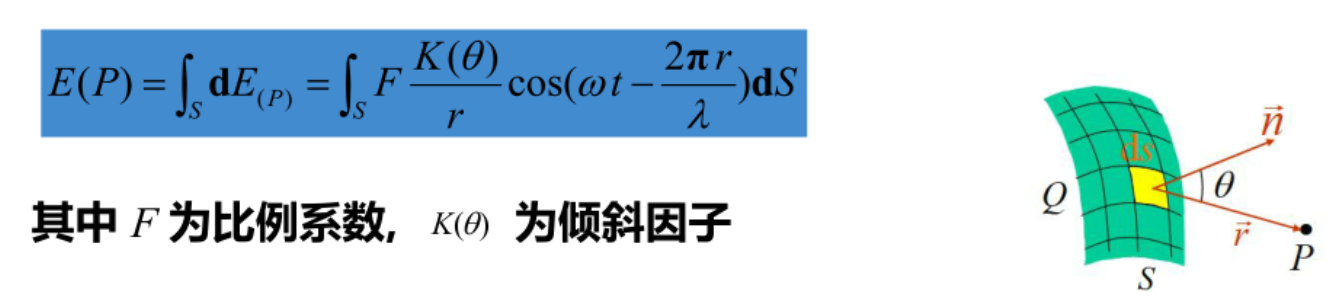
\includegraphics[width=0.55\textwidth]{实验原理示意图_惠更斯-菲涅尔原理.png}
    \caption{惠更斯菲涅尔原理示意图}
\end{figure}
\par

(2)\textbf{单缝衍射光强分布特征}
\par
\begin{figure}[H]
    \centering
    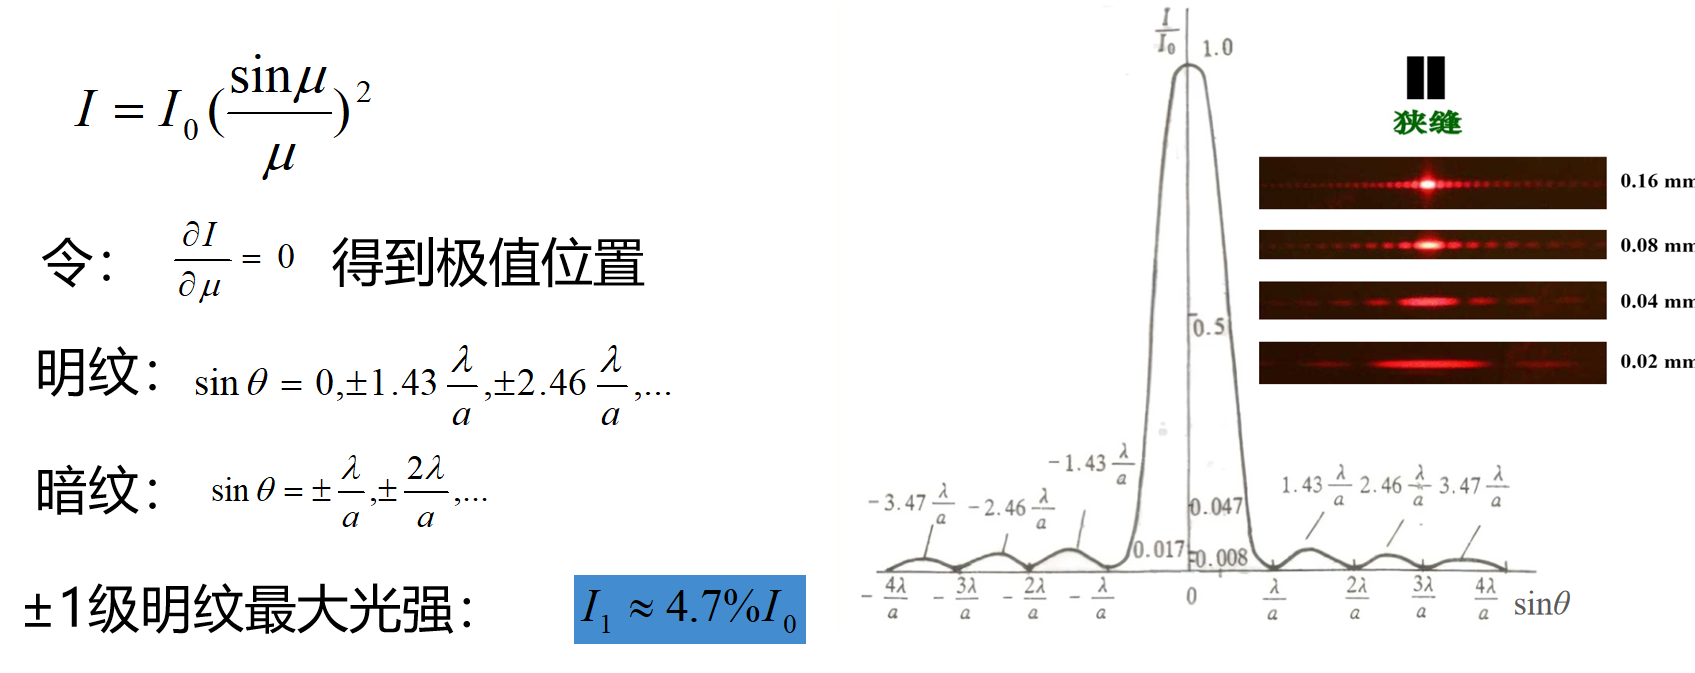
\includegraphics[width=0.55\textwidth]{实验原理示意图_单缝衍射.png}
    \caption{单缝衍射原理示意图}
\end{figure}

(3)\textbf{光栅衍射}
\par
平行光照射投射光栅:同时存在每个缝的单缝衍射和缝与缝间光干涉

\subsection{实验重点(3分)}
(简述本实验的学习重点,不超过100字。)
\subsubsection{理解不同形状衍射物的衍射光强分布特征}

\subsubsection{掌握利用光的衍射法测量微小量的方法}

\subsubsection{了解二维光栅衍射的特征}


\subsection{实验难点(2分)}
(简述本实验的实现难点,不超过100字。)
\par
(1)\textbf{光学器件的精确调节:}需保证光源、单缝、透镜及观察屏等高共轴,微小的偏离会导致衍射条纹畸变或消失,对实验者操作精度要求高。
\par
(2)\textbf{衍射条纹的清晰观察:}环境杂散光易干扰弱光衍射条纹,需在暗室环境下进行,且需调节光源强度和单缝宽度以获得对比度良好的条纹。
\par
(3)\textbf{数据测量的准确性:}条纹位置(如中心到各次级明纹的距离)及单缝与屏间距(D)的测量易受人为读数误差影响,需借助高精度测量工具(如测微目镜)。
\par
(4)\textbf{实验条件的稳定控制:}光源波长稳定性、单缝宽度均匀性及装置振动等因素会影响条纹重复性,需严格控制实验环境。


\begin{fullreportonly}
\section{原始数据(20分)}
(将有老师签名的“自备数据记录草稿纸”的扫描或手机拍摄图粘贴在下方,完整保留姓名,学号,教师签字和日期。)
\begin{figure}[H]
    \centering
    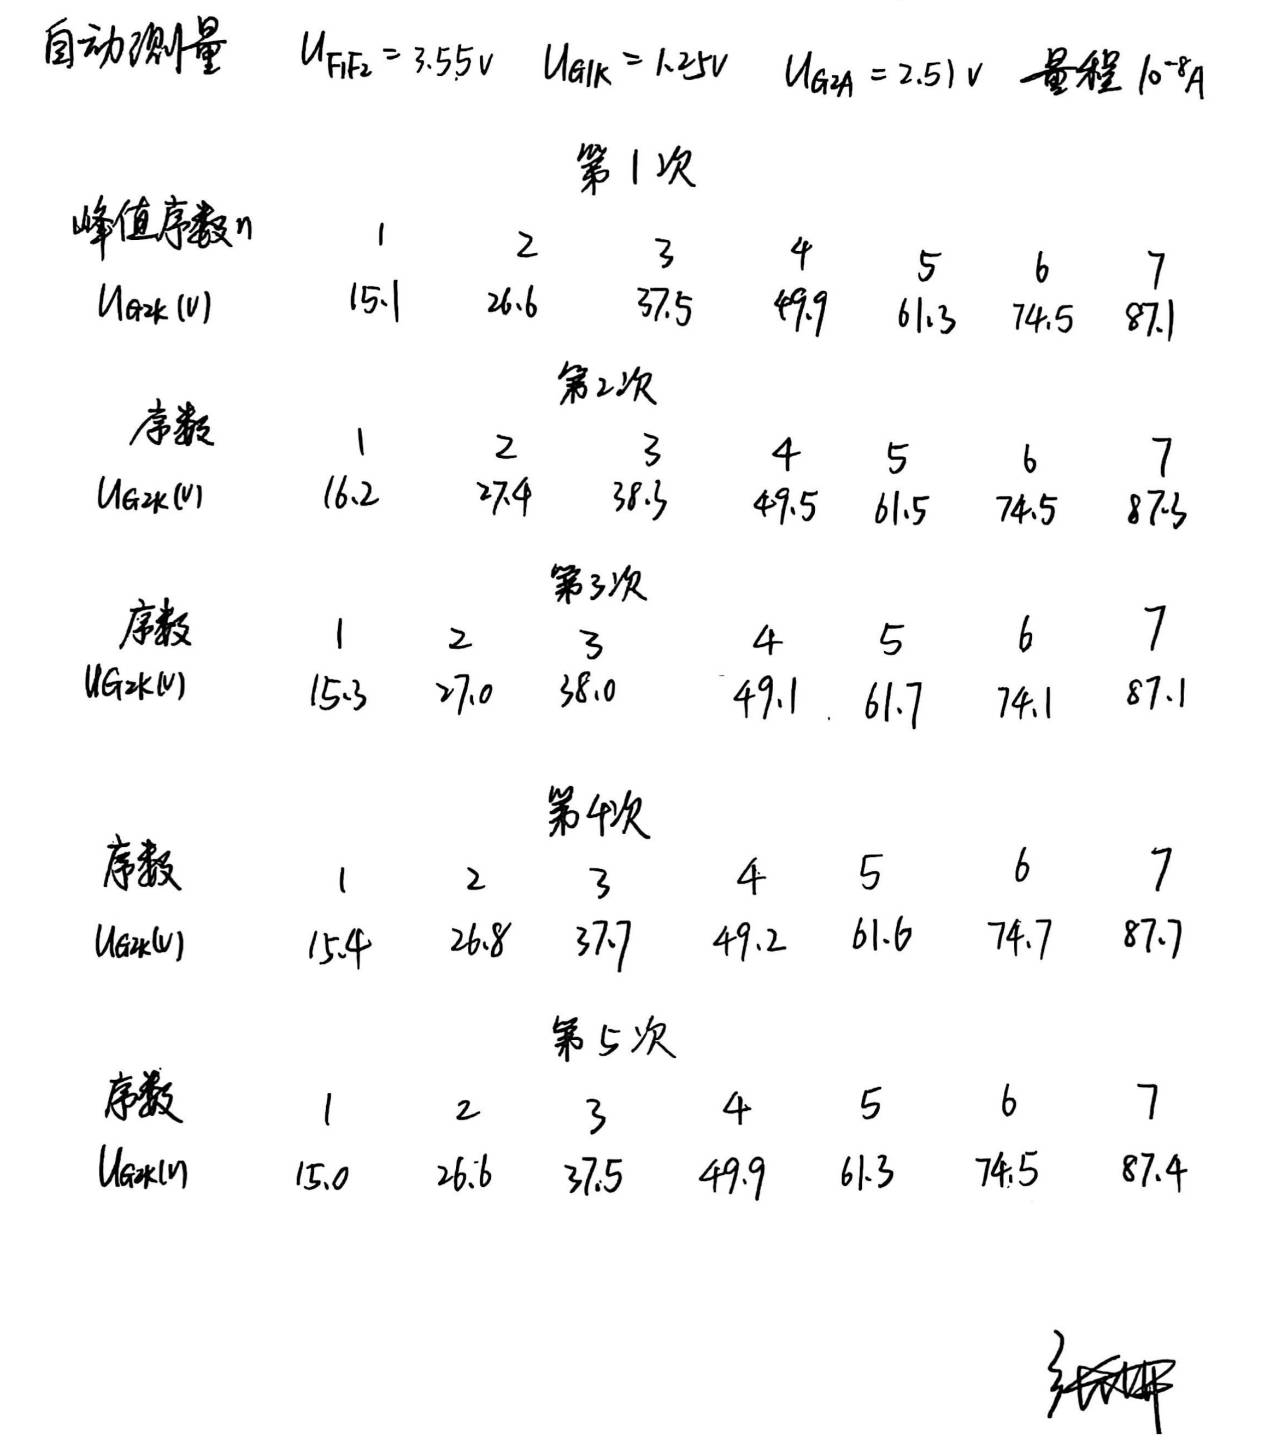
\includegraphics[width=0.55\textwidth]{原始数据1.jpg}
    \caption{实验一原始数据}
\end{figure}

\begin{figure}[H]
    \centering
    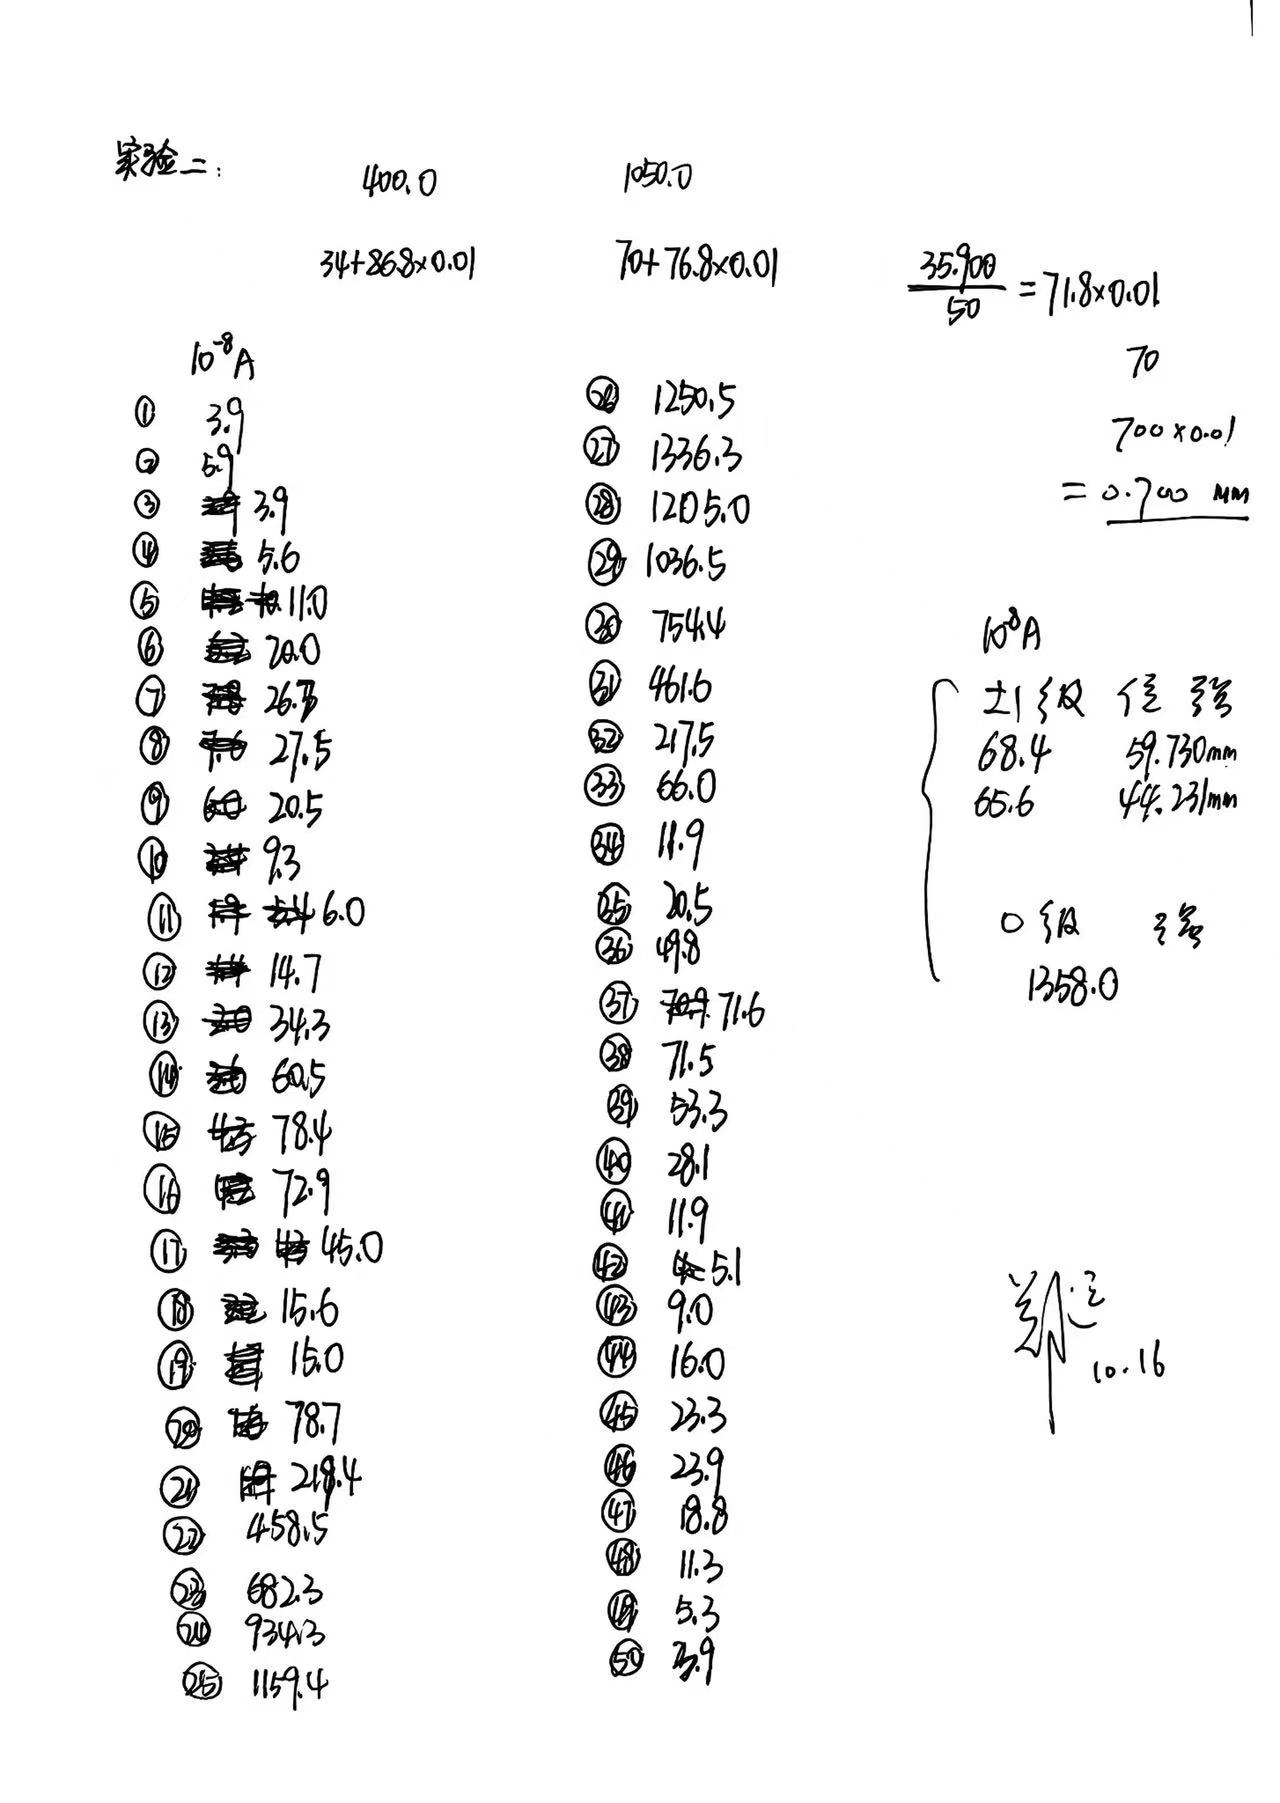
\includegraphics[width=0.55\textwidth]{原始数据2.jpg}
    \caption{实验二原始数据}
\end{figure}

\section{结果与分析(60分)}
\subsection{数据处理与结果(30分)}
(列出数据表格、选择适合的数据处理方法、写出测量或计算结果。)
\subsubsection{实验一:一维光栅}
\begin{table}[H]
    \centering
    \caption{实验一数据处理}
    \begin{tabular}{|c|c|c|c|}
        \hline
        \textbf{光栅位置L1/mm} & 550.0 & \textbf{探测器位置L2/mm} & 1050.0 \\
        \hline
        \textbf{测量次数} & \textbf{-1级亮点位置$x_{-1}$/mm} & \textbf{+1级亮点位置$x_{+1}$/mm} & \textbf{$\Delta x = x_{+1} - x_{-1}$/mm}  \\
        \hline
        1 & 53.450 & 69.390 & 15.940 \\
        \hline
        2 & 53.630 & 69.550 & 15.920 \\
        \hline
        3 & 53.560 & 69.560 & 16.000 \\
        \hline
        4 & 53.550 & 69.582 & 16.032 \\
        \hline
        5 & 53.685 & 69.526 & 15.841 \\
        \hline
        6 & 53.500 & 69.435 & 15.935 \\
        \hline
        \multicolumn{2}{|c|}{$\bar{\Delta L} = L2 - L1 = 500.0mm \quad \bar{\Delta x} = 15.945mm$} & 
        \multicolumn{2}{|c|}{$\sin \theta = \tan \theta = \frac{\bar{\Delta x}}{\bar{\Delta L}} = 0.032$}  \\
        \hline
        \multicolumn{4}{|c|}{根据光栅方程:光的波长$\lambda = (a+b)\sin \theta = 0.02mm \times 0.032 = 0.00064mm = 640.0nm$}  \\
        \hline
        \multicolumn{4}{|c|}{相对误差 = |测量值 - 标准值| / 标准值 = (640 - 635) / 635 = 0.0079}  \\
        \hline
    \end{tabular}
\end{table}
计算得光源波长$\lambda = 640.0nm$

\subsubsection{实验二:单缝}
\begin{table}[H]
    \centering
    \caption{实验二数据处理}
    \begin{tabular}{|c|c|c|c|}
        \hline
        \textbf{光栅位置L1/mm} & 400.0 & \textbf{探测器位置L2/mm} & 1050.0  \\
        \hline
        \textbf{-3级亮点位置$x_{-3}$/mm} & 34.868 & \textbf{+3级亮点位置$x_{+3}$/mm} & 70.768  \\
        \hline
        \multicolumn{4}{|c|}{$ \frac{x_{+3} - x_{-3}}{50} = 0.718 = 71.8 \times 0.01$}  \\
        \hline
        \textbf{相对位置/mm} & \textbf{相对光强/$\mu A$} & \textbf{相对位置/mm} & \textbf{相对光强/$\mu A$}  \\
        \hline
        1 & 3.9 & 26 & 1250.5  \\
        \hline
        2 & 5.9 & 27 & 1336.3  \\
        \hline
        3 & 3.9 & 28 & 1250.0  \\
        \hline
        4 & 5.6 & 29 & 1036.5  \\
        \hline
        5 & 11.0 & 30 & 754.4  \\
        \hline
        6 & 20.0 & 31 & 461.6  \\
        \hline
        7 & 26.7 & 32 & 217.5  \\
        \hline
        8 & 27.5 & 33 & 66.0  \\
        \hline
        9 & 20.5 & 34 & 11.9  \\
        \hline
        10 & 9.3 & 35 & 20.5  \\
        \hline
        11 & 6.0 & 36 & 49.8  \\
        \hline
        12 & 14.7 & 37 & 71.6  \\
        \hline 
        13 & 34.3 & 38 & 71.5  \\
        \hline
        14 & 60.5 & 39 & 53.5  \\
        \hline
        15 & 78.4 & 40 & 28.1  \\
        \hline
        16 & 72.9 & 41 & 11.9  \\
        \hline
        17 & 45.0 & 42 & 5.1  \\
        \hline
        18 & 15.6 & 43 & 9.0  \\
        \hline
        19 & 15.0 & 44 & 16.0  \\
        \hline
        20 & 78.7 & 45 & 23.3  \\
        \hline 
        21 & 219.4 & 46 & 23.9  \\
        \hline
        22 & 458.5 & 47 & 18.8  \\
        \hline
        23 & 682.3 & 48 & 11.3  \\
        \hline
        24 & 934.3 & 49 & 5.3  \\
        \hline
        25 & 1159.4 & 50 & 3.9  \\
        \hline
        \multicolumn{2}{|c|}{0级光强$I_0/\mu A$} &
        \multicolumn{2}{|c|}{1358.0}  \\
        \hline
        \textbf{-1级亮点位置$x_{-1}$/mm} & 44.231 & \textbf{-1级光强/$\mu A$} & 65.6  \\
        \hline
        \textbf{+1级亮点位置$x_{+1}$/mm} & 59.730 & \textbf{+1级光强/$\mu A$} & 68.4  \\
        \hline
        \multicolumn{2}{|c|}{$\pm$ 1级光强 $I_1/\mu A$} &
        \multicolumn{2}{|c|}{ $= \frac{65.6 + 68.4}{2} = 67.0$}  \\
        \hline
    \end{tabular}
\end{table}

(1)\textbf{单缝衍射光强分布特征:}
\begin{figure}[H]
    \centering
    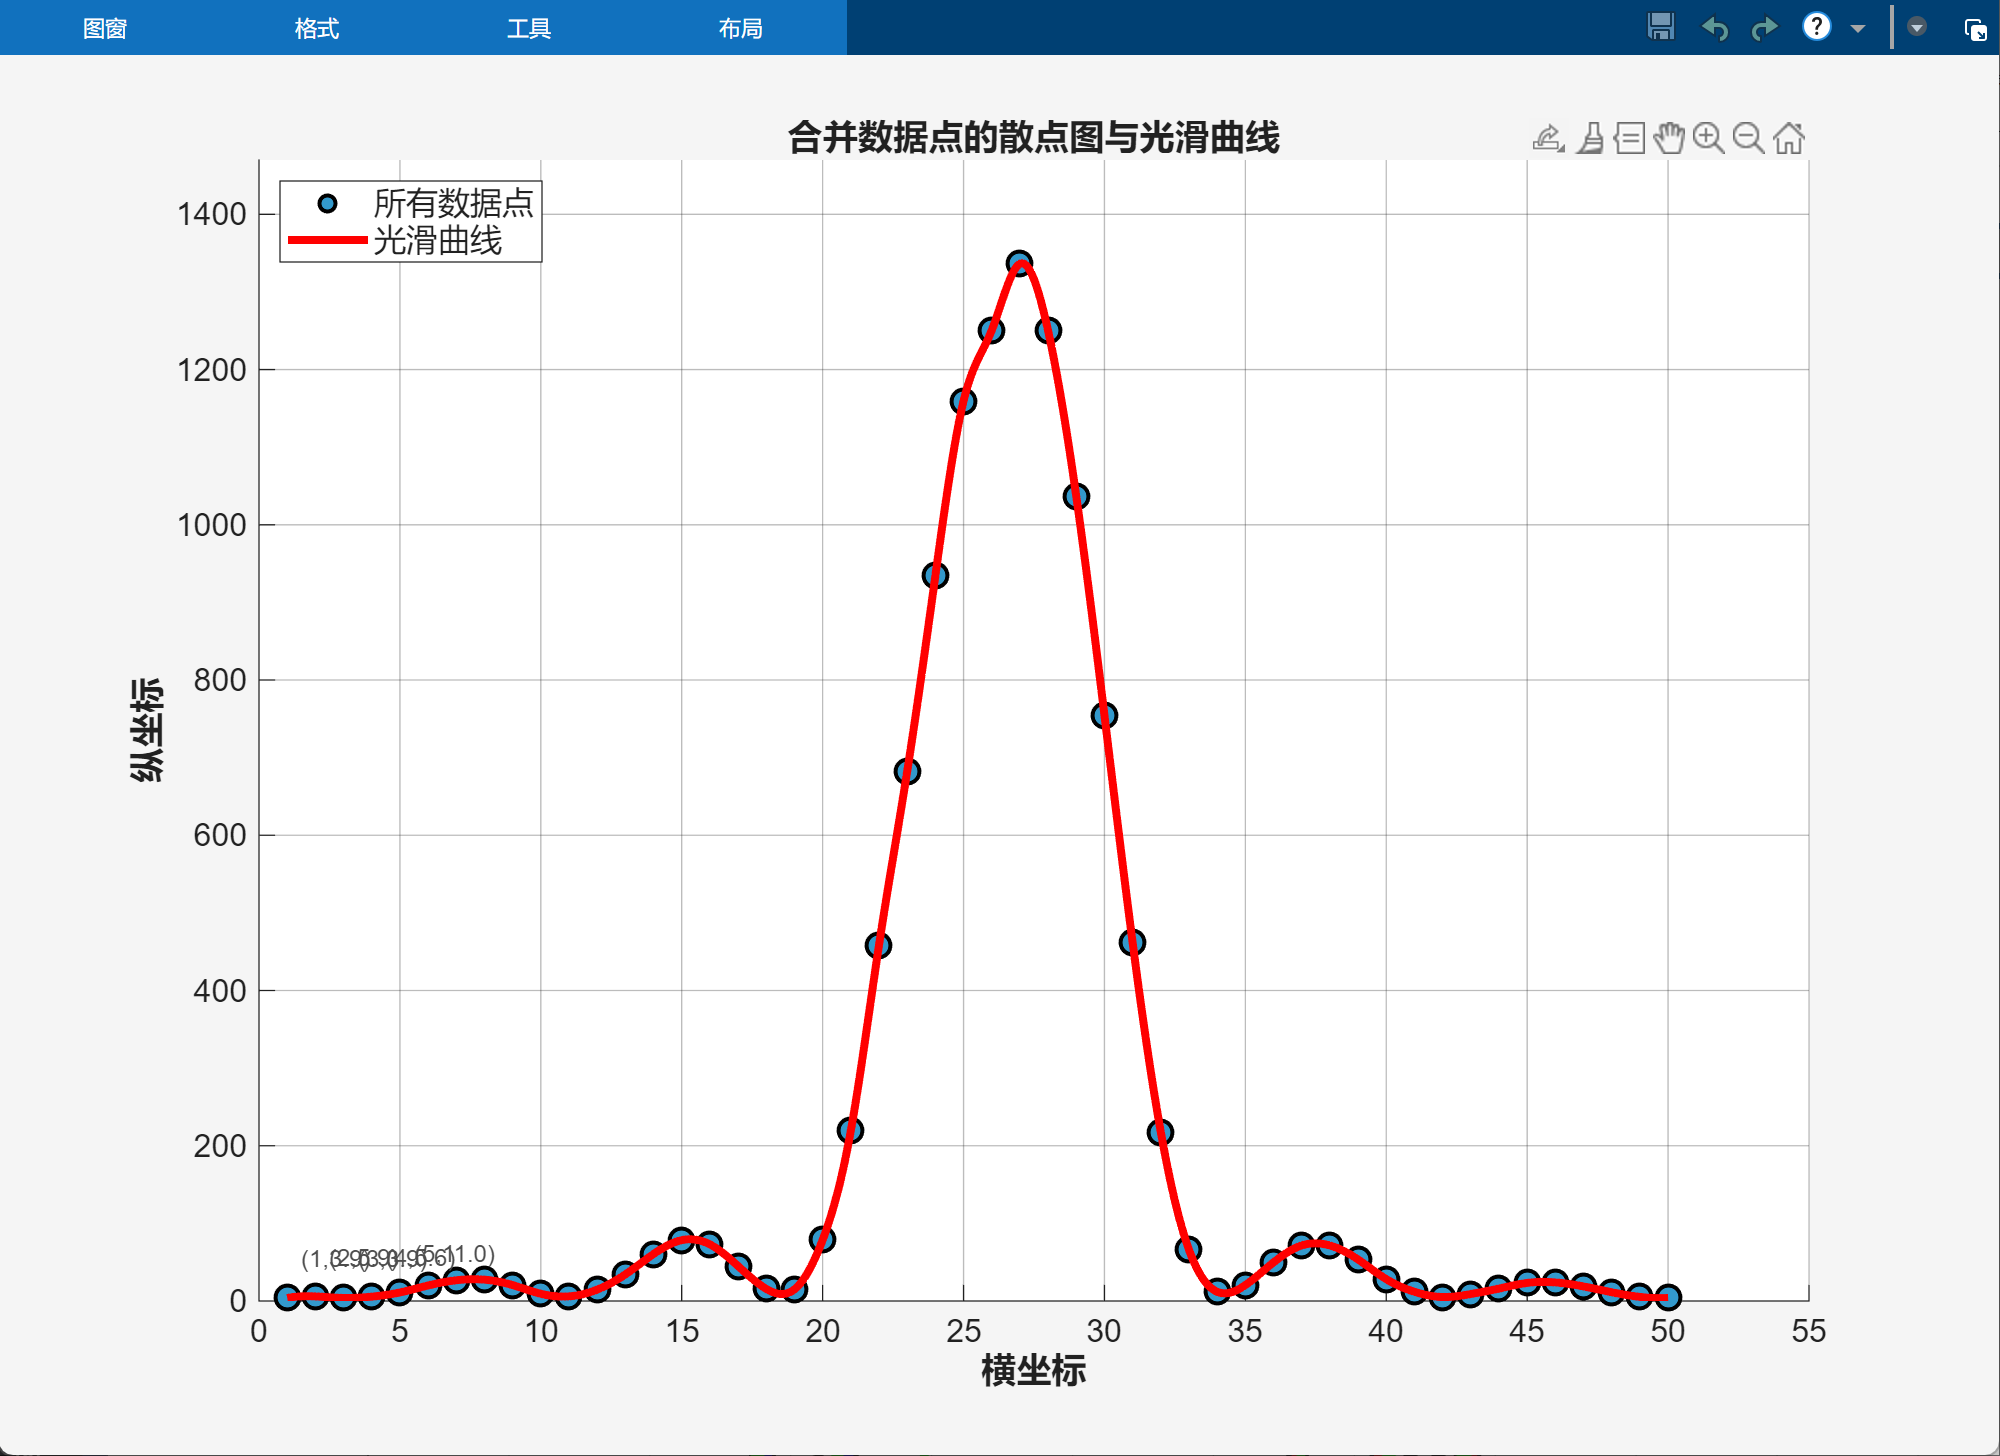
\includegraphics[width=0.70\textwidth]{实验二数据处理.png}
    \caption{单缝衍射光强分布特征}
\end{figure}

(2)\textbf{计算单缝宽度 a}
\par
公式:$\sin \theta = \pm 1.43 \frac{\lambda}{a}$ 由实验一测量结果知:$\lambda = 640.0nm$
\par
$\Delta x = x_{+1} - x_{-1} = 59.730 - 44.231 = 15.499mm \quad \Delta L = L2 - L1 = 1050.0 - 400.0 = 650.0mm$
\par
$\sin \theta = \tan \theta = \frac{\Delta x}{\Delta L} = \frac{15.499}{650.0} = 0.0238$
\par
计算得 $a \approx 38389.26nm \approx 0.038mm$
\par
\vspace{0.5cm}
(3)\textbf{验证光强比:}
\par
$I_1 = 67.0\mu A \quad I_0 = 1358.0\mu A$
\par
光强比$\frac{I_1}{I_0} = 4.93\%$



\subsection{误差分析(20分)}
(运用测量误差、相对误差或不确定度等分析实验结果,写出完整的结果表达式,并分析误差原因。)
\subsubsection{实验一相对误差}
测量值:640.0 \quad 标准值:635.0
\par
相对误差 = |测量值 - 标准值| / 标准值 = (640 - 635) / 635 = 0.79\%

\subsubsection{实验二相对误差}
光强比测量值:4.93\% \quad 标准值:4.7\% 
\par
相对误差 = |测量值 - 标准值| / 标准值 = 4.89\%

\subsubsection{误差来源分析}
(1)\textbf{光学元件}:单缝/光栅边缘不锐利、宽度不均匀,导致衍射条纹强度分布不对称;光栅刻痕间距不均匀或存在缺级;光学元件(透镜、狭缝、接收屏)未共轴,导致光轴偏移,衍射图样偏离接收屏中心或部分被遮挡。
\par

(2)\textbf{光源}:光源强度波动会使条纹清晰度变化,影响读数;光源发出的光未严格准直为平行光(如未通过准直透镜或透镜焦距不准),会使入射光存在发散角,导致衍射条纹间距不均匀或中心偏移。
\par

(3)\textbf{实验操作}:人眼判断条纹极值位置(最暗/最亮)存在主观性,尤其当条纹宽、边缘模糊时,对准中心易产生误差;测量条纹位置的工具(游标卡尺、读数显微镜、测微目镜)存在零点误差或刻度不均匀。
\par

(4)\textbf{环境干扰}:空气流动或温度变化引起折射率波动,影响光程;杂散光(背景光)降低条纹对比度,掩盖弱条纹。
\par

(5)\textbf{理论近似:}单缝衍射中用$\sin \theta \approx \tan \theta \approx \theta$(弧度);实验中用透镜模拟“无穷远光源/接收屏”。


\subsection{实验探讨(10分)}
(对实验内容、现象和过程的小结,不超过100字。)
\par
通过此次实验,我理解了不同形状衍射物的衍射光强分布特征,掌握了利用光的衍射法测量微小量的方法,了解了二维光栅衍射的特征。同时,我在实验中学会了精准调节光路(确保平行光入射、缝/光栅垂直于光轴),使用单色光源(如激光)以保证条纹清晰,观测光强分布;实验后进行合理的数据处理和分析。
\par
该实验锻炼了我的耐心、动手操作能力和数据处理能力,同时对物理学中测量微小量的方法有了更深的认识。

\section{思考题(10分)}
(解答教材或讲义或老师布置的思考题,请先写题干,再作答。)
\subsection{单缝衍射两侧光强不是严格对称的原因}
(1)\textbf{光学元件:}若单缝边缘不锐利、宽度不均匀(如一侧边缘有毛刺或缝宽局部变化),会导致衍射波前分布不对称,使得两侧光强分布差异明显;单缝平面未与入射光严格垂直,或光学系统未完全共轴,导致入射光在单缝两侧的入射角不同,进而引起衍射图样偏移和强度不对称。
\par

(2)\textbf{光源:}光源强度不稳定或存在偏振方向偏差,会导致两侧衍射光能量分布不均衡;扩展光源(非点光源)的光强分布不均也会加剧不对称。
\par

(3)\textbf{实验操作:}若未通过“等高共轴”法精确调节各器件,可能导致光轴倾斜,使得衍射图样偏离接收中心,单侧光强被部分遮挡或衰减。

\subsection{狭缝宽度是否越小越好?为什么?}
否。
\par
(1)\textbf{光强与条纹亮度与狭缝宽度有关:}当狭缝宽度过小时,通过狭缝的光通量显著减少,导致衍射条纹(尤其是高级次条纹)亮度急剧降低,甚至因光强太弱而无法清晰观察或被背景杂散光掩盖,影响实验现象的可观测性。
\par

(2)\textbf{实验误差与实际条件限制:}极窄的狭缝难以保证边缘锐利和宽度均匀,可能导致衍射条纹强度分布不对称(如暗纹模糊、亮纹展宽),偏离理想单缝衍射的光强分布规律。

\subsection{描述一个生活中光的衍射现象,怎么做?现象是什么?}
\textbf{CD/DVD表面的彩色花纹}
\par
现象:当白光照射到光盘表面时,会看到绚丽的彩虹色。
\par
原理:光盘表面布满了密集的、等间距的数据轨道,这些轨道形成了一个“衍射光栅”。当光照射到这些轨道上时,不同颜色的光(波长不同)会发生衍射并相互干涉,使得不同颜色的光被强化到不同的方向,从而将白光分解成我们看到的彩虹光谱。
\end{fullreportonly}
\insertnotes
\end{document}